\documentclass[a4paper,12pt,fleqn]{article}%fleqn pour aligner les equations à gauche
\usepackage{../../Styles/Cours}


\newcommand{\chnum}{Chapitre 12}
\newcommand{\chtitle}{MVT dans un champ uniforme - Analyse}
\newcommand{\dtype}{Cours}
  

\begin{document}
\maketitle

\begin{longtable}{|m{5cm}|m{13cm}|}
\hline
\tabletail{\hline}
\textbf{1. Système et référentiel d'étude}\begin{itemize**}
	\item Définir le système
	\item Choisir un référentiel adapté (avec son repère)
	\item Vérifier qu'il est galiléen
\end{itemize**} & \color {gray}\begin{itemize**} \item Le \textbf{système} étudié est un point matériel ou le centre de masse \textbf{G} d'un corps. \item Son mouvement est étudié dans un \textbf{référentiel} supposé \textbf{galiléen}. \item L'étude se fait dans un \textbf{repère} ($O$, $\vec{i}$,$\vec{j}$, $\vec{k}$) dont l'origine $O$ est choisie au niveau de la position initiale du système.\end{itemize**} \color{black}\\
\hline
\textbf{2. Schéma} \begin{itemize**}
	\item la trajectoire
	\item le repère
	\item les éléments liés aux données de l'énoncé
\end{itemize**} &
\begin{center}
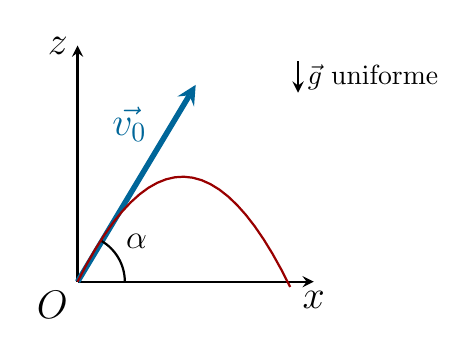
\begin{tikzpicture}
	\node[below left] (O) at (0,0){\Large $O$};
	\draw[thick, -stealth] (0,0) -- (0,3);
	\draw[thick, -stealth] (0,0) -- (3,0);
		
	%\draw[line width = 2pt, -stealth] (0,0) to (1,0);
	%\draw[line width = 2pt, -stealth] (0,0) to (0,1);
	
	\node[left] (y) at (0,3){\Large $z$};
	\node[below] (x) at (3,0){\Large $x$};
		
	%\node[left] (j) at (0,.5){\Large $\vec{j}$};
	%\node[below] (i) at (.5,0){\Large $\vec{i}$};
	
	%\draw[line width = 1.2pt, blue!60!green,-stealth] (-1.2,1) to (-2,2);
	
	\node[left,blue!60!green] (v0) at (1,2){\Large $\vec{v_0}$};
	\node[above] (alpha) at (.75,0.3){\large $\alpha$};
	
	\draw[line width = 2pt, -stealth, blue!60!green] (0,0) to (1.5,2.5);
	
	\draw[thick] (0.6,0) arc (0:60:.6);
	\draw [domain=0:2.7, thick, red!60!black] plot(\x,{-0.75*\x * \x  + 2*\x});
	
	\draw[thick, -stealth] (2.8,2.8) to (2.8,2.4);
	\node[right] (g) at (2.8,2.6){$\vec{g}$ uniforme};
\end{tikzpicture}
\end{center}\\
\hline
\textbf{3. Les forces} \begin{itemize**}
	\item lister la ou les forces s'exerçant sur le système
	\item la ou les représenter sur le schéma précédent
\end{itemize**} & Bilan des forces : \begin{itemize**} \item $\vec{P}$ uniquement car chute libre \end{itemize**} \begin{center}
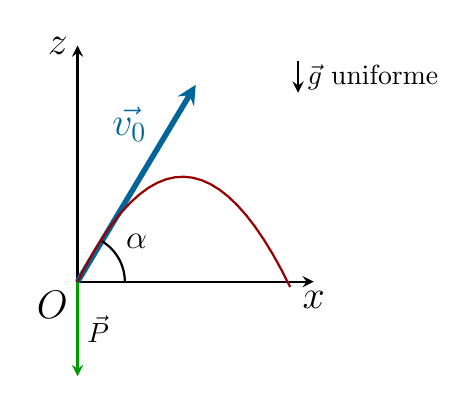
\begin{tikzpicture}
	\node[below left] (O) at (0,0){\Large $O$};
	\draw[thick, -stealth] (0,0) -- (0,3);
	\draw[thick, -stealth] (0,0) -- (3,0);
		
	%\draw[line width = 2pt, -stealth] (0,0) to (1,0);
	%\draw[line width = 2pt, -stealth] (0,0) to (0,1);
	
	\node[left] (y) at (0,3){\Large $z$};
	\node[below] (x) at (3,0){\Large $x$};
		
	%\node[left] (j) at (0,.5){\Large $\vec{j}$};
	%\node[below] (i) at (.5,0){\Large $\vec{i}$};
	
	%\draw[line width = 1.2pt, blue!60!green,-stealth] (-1.2,1) to (-2,2);
	
	\node[left,blue!60!green] (v0) at (1,2){\Large $\vec{v_0}$};
	\node[above] (alpha) at (.75,0.3){\large $\alpha$};
	
	\draw[line width = 2pt, -stealth, blue!60!green] (0,0) to (1.5,2.5);
	
	\draw[thick] (0.6,0) arc (0:60:.6);
	\draw [domain=0:2.7, thick, red!60!black] plot(\x,{-0.75*\x * \x  + 2*\x});
	
	\draw[thick, -stealth] (2.8,2.8) to (2.8,2.4);
	\node[right] (g) at (2.8,2.6){$\vec{g}$ uniforme};
	
	\draw[green!60!black,thick, -stealth] (0,0) to (0,-1.2);
	\node[right] (g) at (0,-0.6){$\vec{P}$};
\end{tikzpicture}
\end{center}\\ \hline
\textbf{4. Deuxième loi de Newton et vecteur accélération} \begin{itemize**}
	\item énoncer la deuxième loi de Newton
	\item l'appliquer en projetant les vecteurs forces sur chaque axe du repère
	\item en déduire les coordonnées du vecteur accélération
\end{itemize**} & D'après la deuxième loi de Newton, $ \sum \vec{F} = m \cdot \vec{a}$ $$\vec{P} = m \cdot \vec{a}$$
$$\Leftrightarrow m \cdot \vec{g} = m \cdot \vec{a} $$
$$\Leftrightarrow \vec{g} = \vec{a} $$
Le vecteur accélération est égal au vecteur champ de pesanteur. On en déduit ses coordonnées : \begin{eqnarray}
	\vec{a}(t) \left\lbrace \begin{aligned}
	a_x(t) = 0\\
	a_y(t) = 0\\
	a_z(t) = -g\\	
	\end{aligned} \right\rbrace\nonumber
\end{eqnarray} \\
\hline
\textbf{5. Vecteur vitesse} \begin{itemize**}
	\item intégrer les coordonnées du vecteur accélération
	\item utiliser les conditions initiales pour déterminer les constantes
\end{itemize**} & Le vecteur accélération est la dérivée du vecteur vitesse. Donc le vecteur vitesse est la \textbf{primitive} du vecteur accélération. Pour trouver les coordonnées de $\vec{v}$, on \textbf{intègre} les coordonnées de $\vec{a}$.
\begin{eqnarray}
	\vec{a}(t) \left\lbrace \begin{aligned}
	a_x(t) = \frac{dv_x}{dt} =0\\
	a_y(t) = \frac{dv_y}{dt} =0\\
	a_z(t) = \frac{dv_z}{dt} = -g\\	
	\end{aligned}
	\right\rbrace \rightarrow 	
	\vec{v}(t) \left\lbrace \begin{aligned}
	v_x(t) = cste_1\\
	v_y(t) = cste_2\\
	v_z(t) = -gt + cste_3\\	
	\end{aligned} \right\rbrace \nonumber
\end{eqnarray}
Pour trouver les valeurs des constantes, on utilise les \textbf{conditions initiales} ($t=0~s$).
\begin{itemize**}
	\item d'après le schéma  :
\begin{eqnarray}
	\vec{v_0} \left\lbrace \begin{aligned}
	v_{0x}(t) = v_0 \cdot \cos \alpha\\
	v_{0y}(t) = 0\\
	v_{0z}(t) = v_0 \cdot \sin \alpha\\	
	\end{aligned} \right\rbrace \nonumber
\end{eqnarray}
	\item d'après les coordonnées ci-dessous :
\begin{eqnarray}
	\vec{v_0} = \vv{v(0)} \left\lbrace \begin{aligned}
	cste_1\\
	cste_2\\
	-g \times 0 + cste_3\\	
	\end{aligned} \right\rbrace \nonumber
\end{eqnarray}\end{itemize**}
donc :
\begin{eqnarray}
	\begin{aligned} cste_1 = v_0 \cdot \cos \alpha \nonumber \\
	cste_2 = 0 \nonumber \\
	cste_3 = v_0 \dot \sin \alpha  \nonumber \end{aligned}
\end{eqnarray}
On en déduit :
\begin{eqnarray}
	\vec{v}(t) \left\lbrace \begin{aligned}
	v_x(t)=v_0 \cdot \cos \alpha\\
	v_y(t) = 0\\
	v_z(t) = -gt + v_0 \sin \alpha\\
	\end{aligned}\right\rbrace \nonumber
\end{eqnarray}
\\
\hline
\textbf{6. Vecteur position = équations horaires} \begin{itemize*}
	\item intégrer les coordonnées du vecteur vitesse
	\item utiliser les conditions initiales (coordonnées de $\vv{OM}$ à $t=0$) pour déterminer les constantes
\end{itemize*} & Le vecteur vitesse est la dérivée su vecteur position. Donc le vecteur position est la \textbf{primitive} du vecteur vitesse. Pour trouver les coordonnées de $\vec{v}$, on \textbf{intègre} les coordonnées de $\vec{v}$.
\begin{eqnarray}
	\vec{v}(t) \left\lbrace \begin{aligned}
	v_x(t)=\frac{dx}{dt} = v_0 \cdot \cos \alpha \\
	v_y(t) = \frac{dy}{dt} =  0 \\
	v_z(t) = \frac{dz}{dt} = -gt + v_0 \sin \alpha
	\end{aligned} \right\rbrace \nonumber
\end{eqnarray}
\begin{eqnarray}
	\rightarrow 
	\vv{OM}(t) \left\lbrace \begin{aligned}
	x(t)=(v_0 \cdot \cos \alpha)t + cste_4 \\
	y(t) = cste_5 \\
	z(t) = -\frac{1}{2} gt^2 + (v_0 \sin \alpha)t + cste_6
	\end{aligned} \right\rbrace \nonumber
\end{eqnarray}
Pour trouver les valeurs des constantes, on utilise les \textbf{conditions initiales} ($t=0~s$).
\begin{itemize**}
	\item À $t=0~s$, $x_0 = y_0 =z_0 = 0$ donc :
\begin{eqnarray}
	\vv{OM}(0) \left\lbrace \begin{aligned}
	x(t)=(v_0 \cdot \cos \alpha) \times 0 + cste_4 =0 \\
	y(t) = cste_5 =0 \\
	z(t) = -\frac{1}{2} g\times 0^2 + (v_0 \sin \alpha)\times 0 + cste_6 =0
	\end{aligned} \right\rbrace \nonumber
\end{eqnarray}
soit $cste_4 = cste_5 =cste_6 =0$
	\item On en déduit les \textbf{équations horaires} :
\begin{eqnarray}
	\vv{OM}(t) \left\lbrace \begin{aligned}
	x(t)=(v_0 \cdot \cos \alpha)t\\
	y(t) = 0 \\
	z(t) = -\frac{1}{2} gt^2 + (v_0 \sin \alpha)t
	\end{aligned} \right\rbrace \nonumber
\end{eqnarray}
\end{itemize**}
\\
\hline
\multicolumn{2}{|m{18cm}|}{La coordonnée $y$ est constamment nulle, donc la trajectoire du centre de masse du système est \textbf{plane}. À l'avenir, on pourra donc simplifier l'étude d'un tel mouvement en ne conservant que deux directions dès le début de la démarche. À la suite de cette étude, il est possible de déterminer l'\textbf{'équation de la trajectoire}, c'est-à-dire la relation mathématique entre différentes coordonnées su système, par exemple l'expression de $z$ en fonction de $x$.}\\ \hline
\textbf{7. Équation de la trajectoire} \begin{itemize*}
	\item isoler $t$ dans l'équation horaire la plus simple
	\item remplacer $t$ dans la deuxième équation horaire et simplifier
\end{itemize*} & \begin{itemize**}
	\item On isole $t$ dans l'équation horaire x(t) :
	\begin{eqnarray}
		x(t)=(v_0 \cos \alpha)t \nonumber \\
		t=\frac{x}{v_0 \cos \alpha} \nonumber
	\end{eqnarray}
	\item On remplace $t$ dans l'équation horaire $z(t)$ :
	\begin{eqnarray}
		z(x) = -\frac{1}{2}g \cdot \left(\dfrac{x}{v_0 \cos \alpha}\right)^2 + v_0 \cdot \sin \alpha \cdot \frac{x}{v_0 \cos \alpha} \nonumber \\
		z(x) = -\frac{1}{2} \cdot \left(\dfrac{gx^2}{v_0 \cos \alpha}\right)^2 + (\tan \alpha) x \nonumber
	\end{eqnarray}
	On obtient ainsi l'\textbf{équation de la trajectoire}. C'est un polynôme du second degré, donc la trajectoire est une parabole.
\end{itemize**}\\
\hline
\end{longtable}
\end{document}